\documentclass[11pt]{article}
\usepackage{amsmath,amssymb}
\usepackage{natbib}
\usepackage[hmargin=2cm,vmargin=4cm]{geometry}
\usepackage{color}
\usepackage{graphicx,wrapfig,lipsum}

\usepackage{titling}

\setlength{\droptitle}{-11em}   % This is your set screw

\title{Energy Disaggregation using Non-Intrusive Load Monitoring}

\author{Thibaut \textsc{Perol}\\ \small Harvard John A. Paulson School of Engineering and Applied Sciences\\
\textit{Advisors}: James R. Rice and Marine Denolle}
\date{}
\begin{document}
\maketitle


\section{Abstract}

\section{Introduction}
Energy disaggregation is the procedure that infers the energy consumption of appliances in a household given the total energy consumption from a single meter of that household. In recent years, this field has become increasingly popular as smart meters have begun to deploy and are installed in many households across the world, providing energy consumption data at high temporal resolution. This high resolution data enables the use of computer algorithms to estimate the energy consumption of each appliance in the household without having to install meters on individual appliances (hence, non-intrusive load monitoring). Appliance-specific energy consupmtion information can be provided to homeowners to encourage adoption of energy efficiency habits and identify the appliances that would result in the most cost savings if replaced with more energy efficient ones. From the electric utility's perspective, the appliance specific information can be used for demand-response programs and also provide information about how their customers are using electricity within their homes. 

Research on NILM began in the 1980s with Hart, 1985. In these earlier methods, the patterns in electricity consumption of different appliances were identified by humans and these hand-designed feature extractors were then applied to the aggregate signals. Later works \citep{Kelly} developed methods to automatically identify appliances and perform disaggregation. The technology has also been monetized by several startups (eg. Bidgeley, PlotWatt). 

Several data sets have been released for the purpose of comparing disaggregation methods. The Reference Energy Disaggregation Dataset (REDD) \citep{REDD} was released in 2011 from MIT. It includes data from 6 houses spaning a period of 3-19 days for each house and contains sub-metered (appliance-level) data for each household. The Smart* dataset was released in 2012, with sub-metered data for one household and aggregate data for 3 households over a period of 3 months. Most recently, the UK-DALE datset was released in 2014, with 3-17 months of data for 4 households with appliance-level submeters. Due to the cost and intrusiveness of installing appliance-level meters, these datasets tend to have only a few households or span a short period of time. Additionally, the datasets are differently formatted depending on the research group that collected the data, making comparisons among different datasets difficult.  

In an attempt to standardize comparison of different disaggregation methods, \citet{Batra} released the Non-intrusive Load Monitoring Toolkit (NILMTK). NILMTK is an open-source toolkit that provides tools for data processing and evaluation metrics. NILMTK also provides two benchmark disaggregation algorithms, combinatorial optimization (CO) and factorial hidden markov model (FHMM). 

In this project, we compare a new approach using convolutional neural networks against the standard CO and FHMM implementations in NILMTK. 

\section{Methods}
\subsection{Data processing}
We use the REDD dataset, which contains data aggregated and sub-metered data from 6 houses. We use the functions provided in \verb NILMTK  to read in the data. In the figure below, we show the aggregated energy consumption of a household (building 2) over a 13 day period as well as the times each individual appliance was on during a period of 1 day.\\  
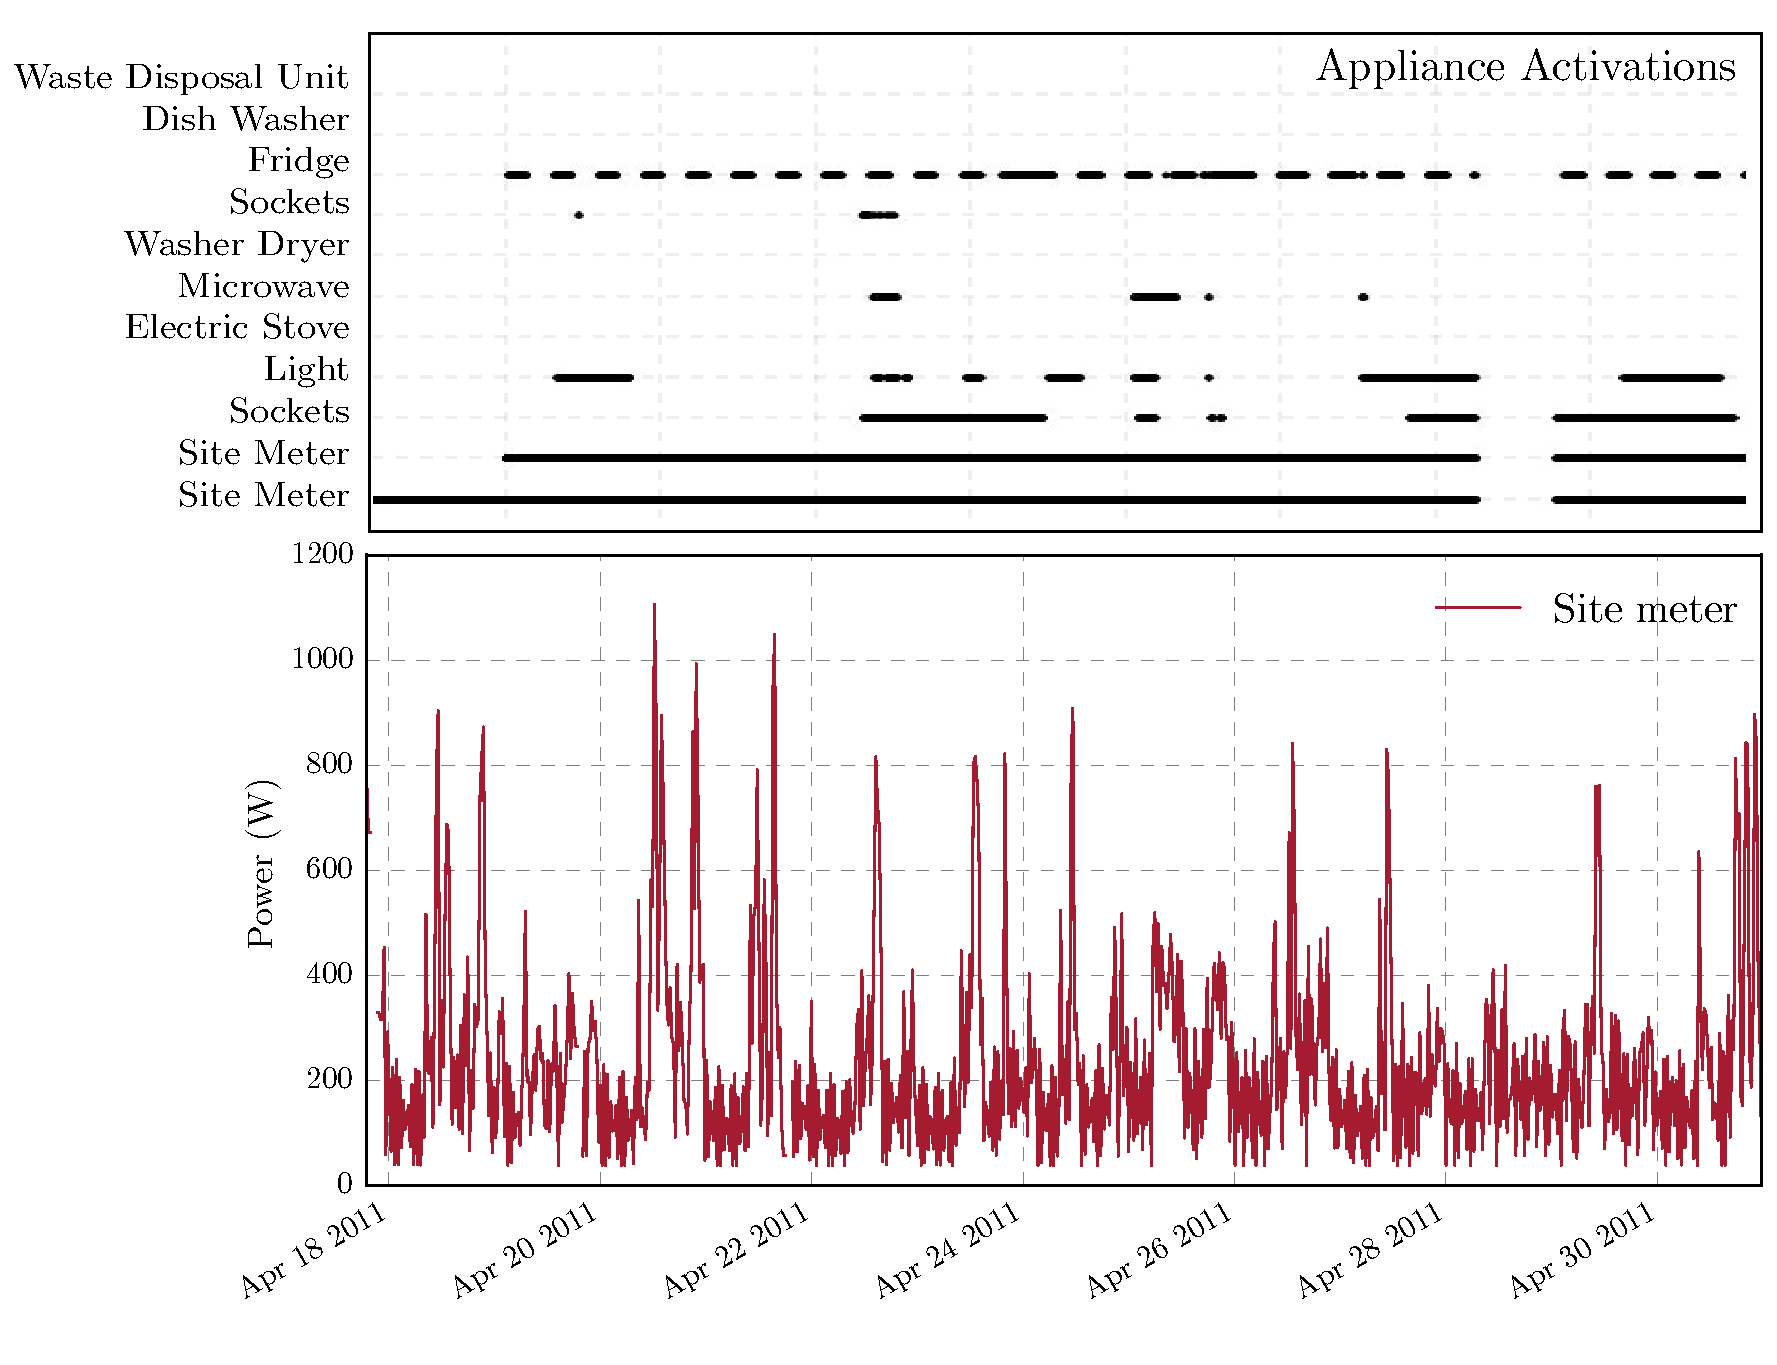
\includegraphics[width=0.6\paperwidth]{../figures/Site_Meter.pdf}

The data is organized by buildings. Within each building, we can get the electricity meter readings using the \verb .elec  attribute. The \verb .mains  sub-meters refer to the aggregated readings. We can refer to each appliance by giving the appliance as a keyword to \verb data.buildings[building_num].elec[appliance] . Some typical appliances in these households include refrigerators, washter dryers, lights, dish washers, microwaves, and sockets. We decided to use fridge and microwave as the two appliances for which we determine the power consumption because they are used in most households (buildings 1, 2, 3, 5).

The data pipeline is shown in the following diagram \\
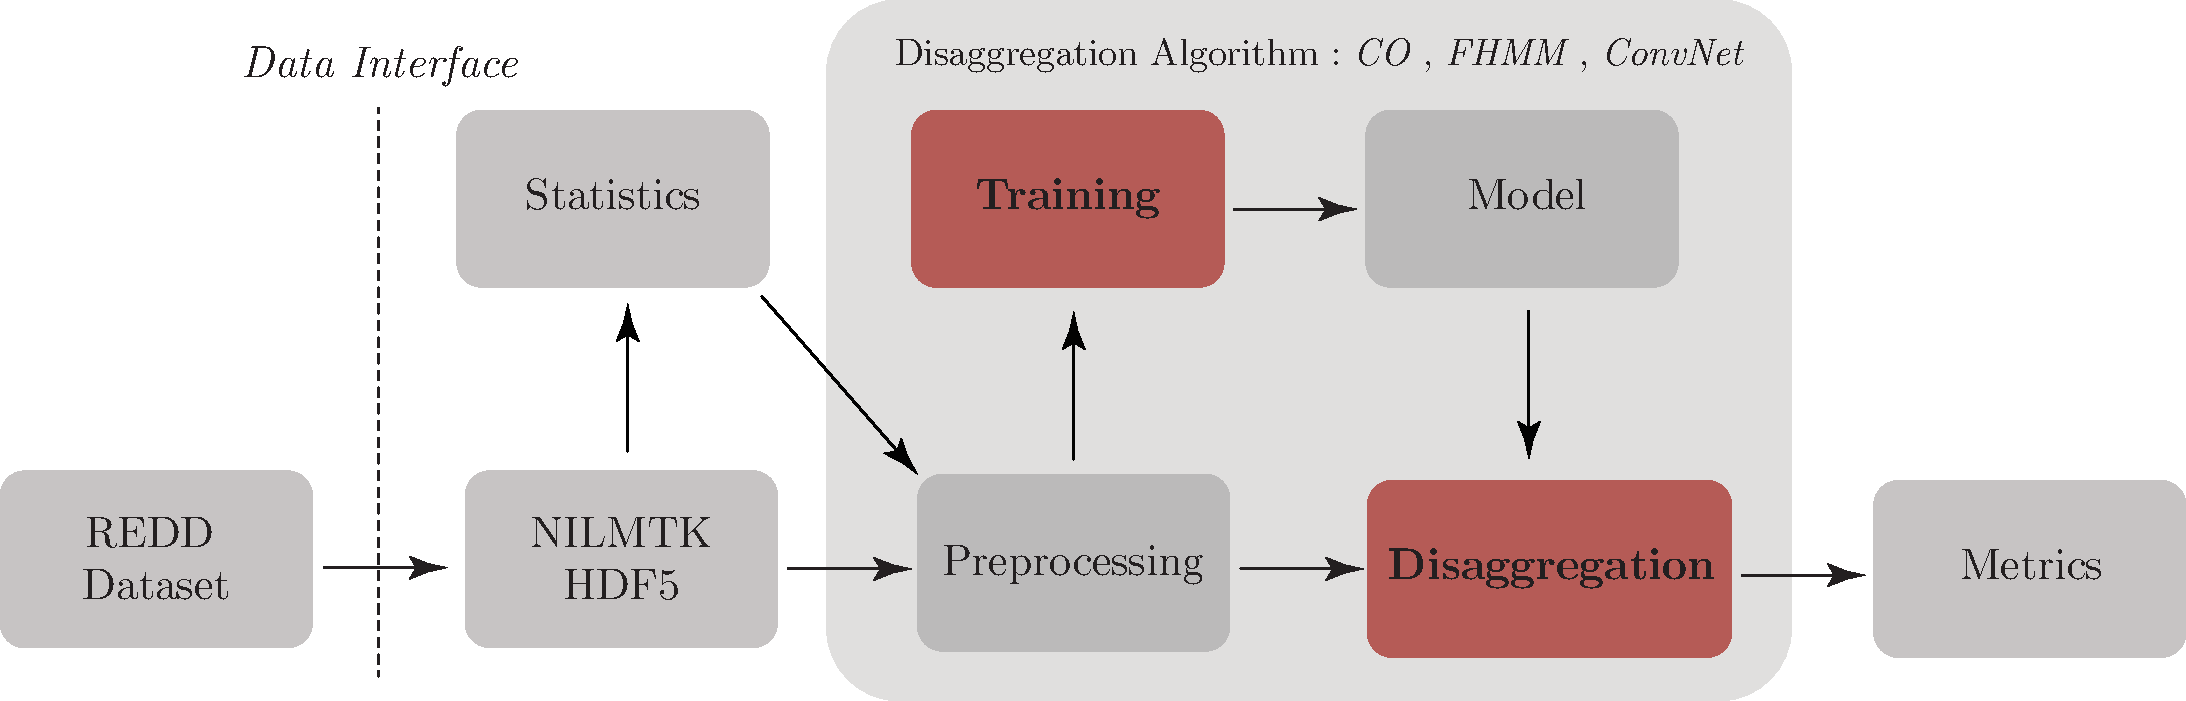
\includegraphics[width=0.6\paperwidth]{../figures/NILM_Data_Pipeline.pdf}

The REDD dataset if first converted to HDF5 format. \verb NILMTK  provides functions to compute statistcs on the dataset as well as preprocessing algorithms. The data from individual meters is then fed into the model for training. After training, the aggregated data can then be fed into the model for disaggregation. \verb NILMTK  also provides functions for computing metrics of how well each disaggregation algorithm performs.

\subsection{Combinatorial Optimization}
\subsection{Factorial Hidden Markov Model}
Factorial hidden markov models (FHMM) are an extension to hidden markov models (HMM) where the hidden state is factored into multiple state variables \citep{Ghahraani}. In a hidden markov model, the observed states of the system are the aggregated power consumption of the household. The hidden states are the states of each appliance. This is shown in the diagram below. \\ 
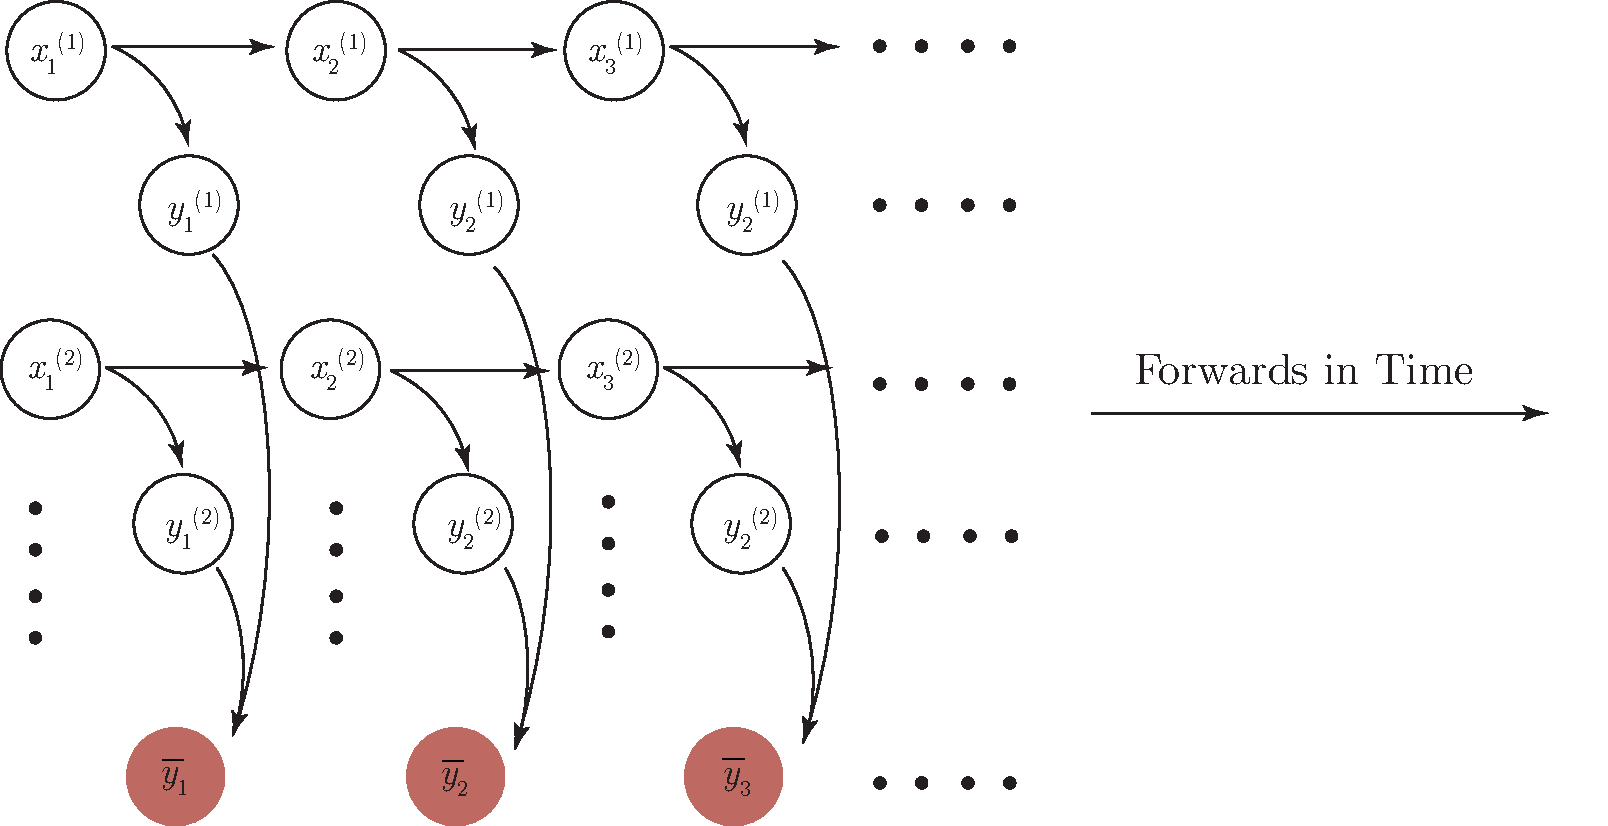
\includegraphics[width=0.4\textwidth]{../figures/FHMM.pdf}

In the above diagram, $y_t$ is the observed state (aggregate power consumption) at time $t$, $y_t^{(i)}$ is the power consumption of appliance $i$ at time $t$ (used only in training), and $x_t^{(i)}$ is the hidden state of appliance $i$ at time $t$. Since the observed state is continuous, the emission probabilities are modeled with a Gaussian distribution: 
\[P(y_t|x_t^{(1:N)}) = \mathcal{N} \left(\sum_{i=1}^N \mu^{(i)}, \Sigma \right) \]
where the mean is the sum of the means of the individual appliances. The transition probabilities can be factored as
\[P(x_t^{1:N)}|x_{t-1}^{(1:N)}) = \prod_{i=1}^{N} P(x_t^{(i)}|x_{t-1}^{(i)})\]
and the transition probabilities for each individual appliance follow a multinomial distribution. The model also needs an initial probability distribution, $\pi_0$ which also follows a multinomial probability distribution.  

In the NILMTK implementation, the \verb train_across_buildings  function takes as input the sub-metered data for each house, a list of the appliances we want to train for, and a list of the houses we want to include in the training set. The sub-metered data for each appliance is then combined into an array that includes all training houses. An HMM with Gaussian emissions is built for each appliance using the \verb GaussianHMM  function in the \verb hmmlearn  package. The parameters (transition and emission probabilities) for this HMM is then trained using the \verb fit  function from \verb hmmlearn , which uses expectation-maximization (EM) to find the optimal parameters. In the original NILMTK implementation, there are two hidden states for each appliance to represent on and off states. We show results using this implementation as well as with a third state to represent an intermediate level of power consumption (such as spin vs. fill cycles of a washing machine). 

Once these parameters are fit for all appliances, they are combined to form the FHMM. The FHMM has a hidden state for every possible combination of states. To create the combined emission matrix, the mean power consumption for each appliance is summed (if the fridge comsumes 0.5W while off and 150W while on, and a microwave consumes 3 W while off and 350 W while on, then the states would be 3.5 W for both devices off, 153 W for fridge on, microwave off, 350.5W for fridge off, microwave on, and 500 W for both devices on). To create the combined transition matrix, we take the product of the transition probabilities of individual appliances. A new \verb GaussianHMM  model is created using these combined parameters. 

To disaggregate (infer the hidden states), the \verb predict  function of \verb hmmlearn  is used, which has the option of using the Viterbi algorithm or maximum a posteriori (MAP) to decode the most likely state sequence.  
 
\subsection{Convolutional Neural Network}

\section{Results}

\section{Conclusion}



\bibliographystyle{agufull08}
\bibliography{/Users/thibaut/Dropbox/Biblio/Perol_biblio}

\end{document}
